\section{Evidencias de Funcionamiento}

\subsection{Registro del Montaje Físico y Dashboard}
En la Figura~\ref{fig:evidencias_visuales} se presentan el esquema del prototipo físico en protoboard y la interfaz gráfica implementada en Node-RED Dashboard 2.0.

\begin{figure}[H]
    \centering
    \begin{subfigure}[b]{0.48\textwidth}
        \centering
        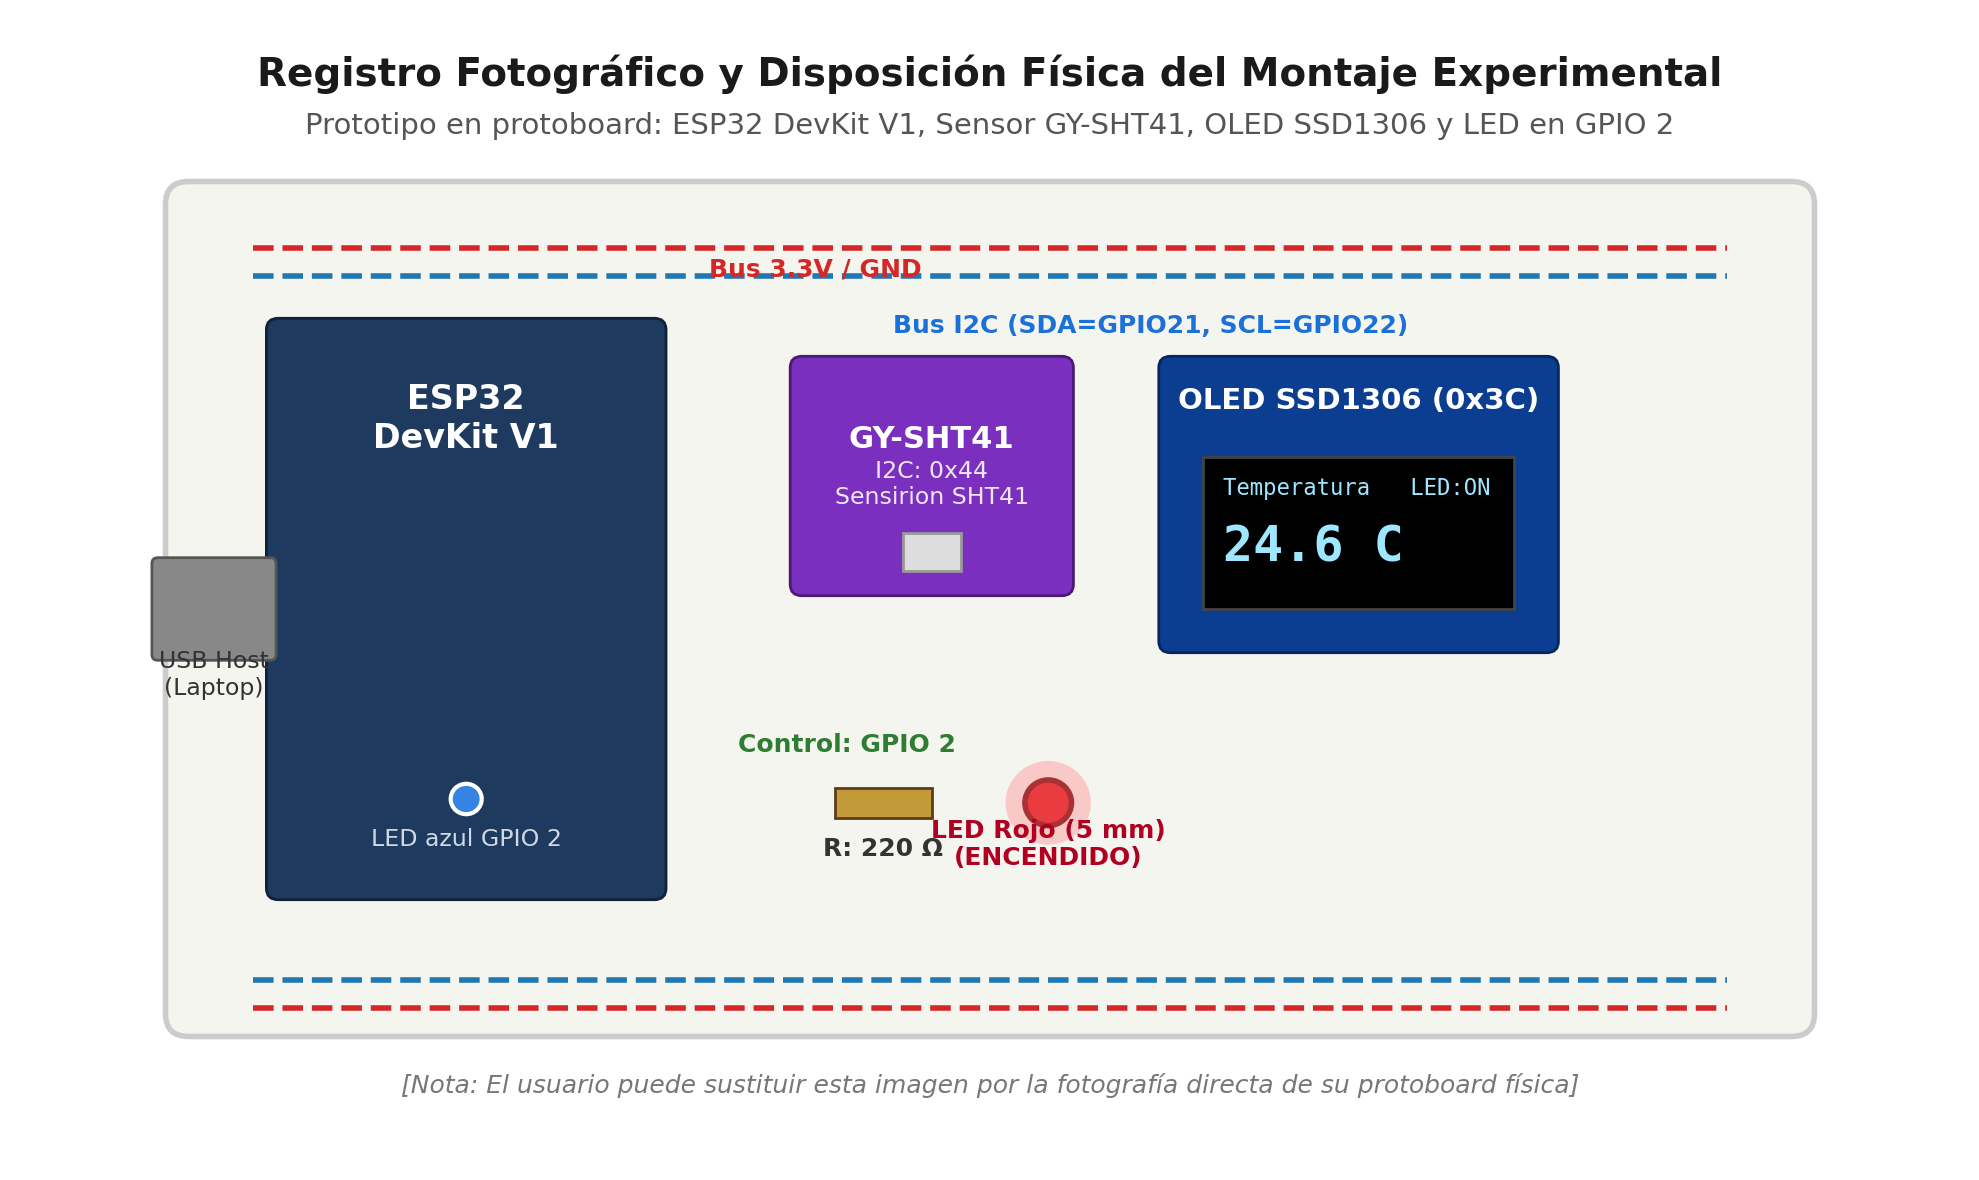
\includegraphics[width=\textwidth]{imagenes/evidencia_montaje_protoboard.png}
        \caption{Montaje experimental en protoboard.}
        \label{fig:sub_montaje}
    \end{subfigure}
    \hfill
    \begin{subfigure}[b]{0.48\textwidth}
        \centering
        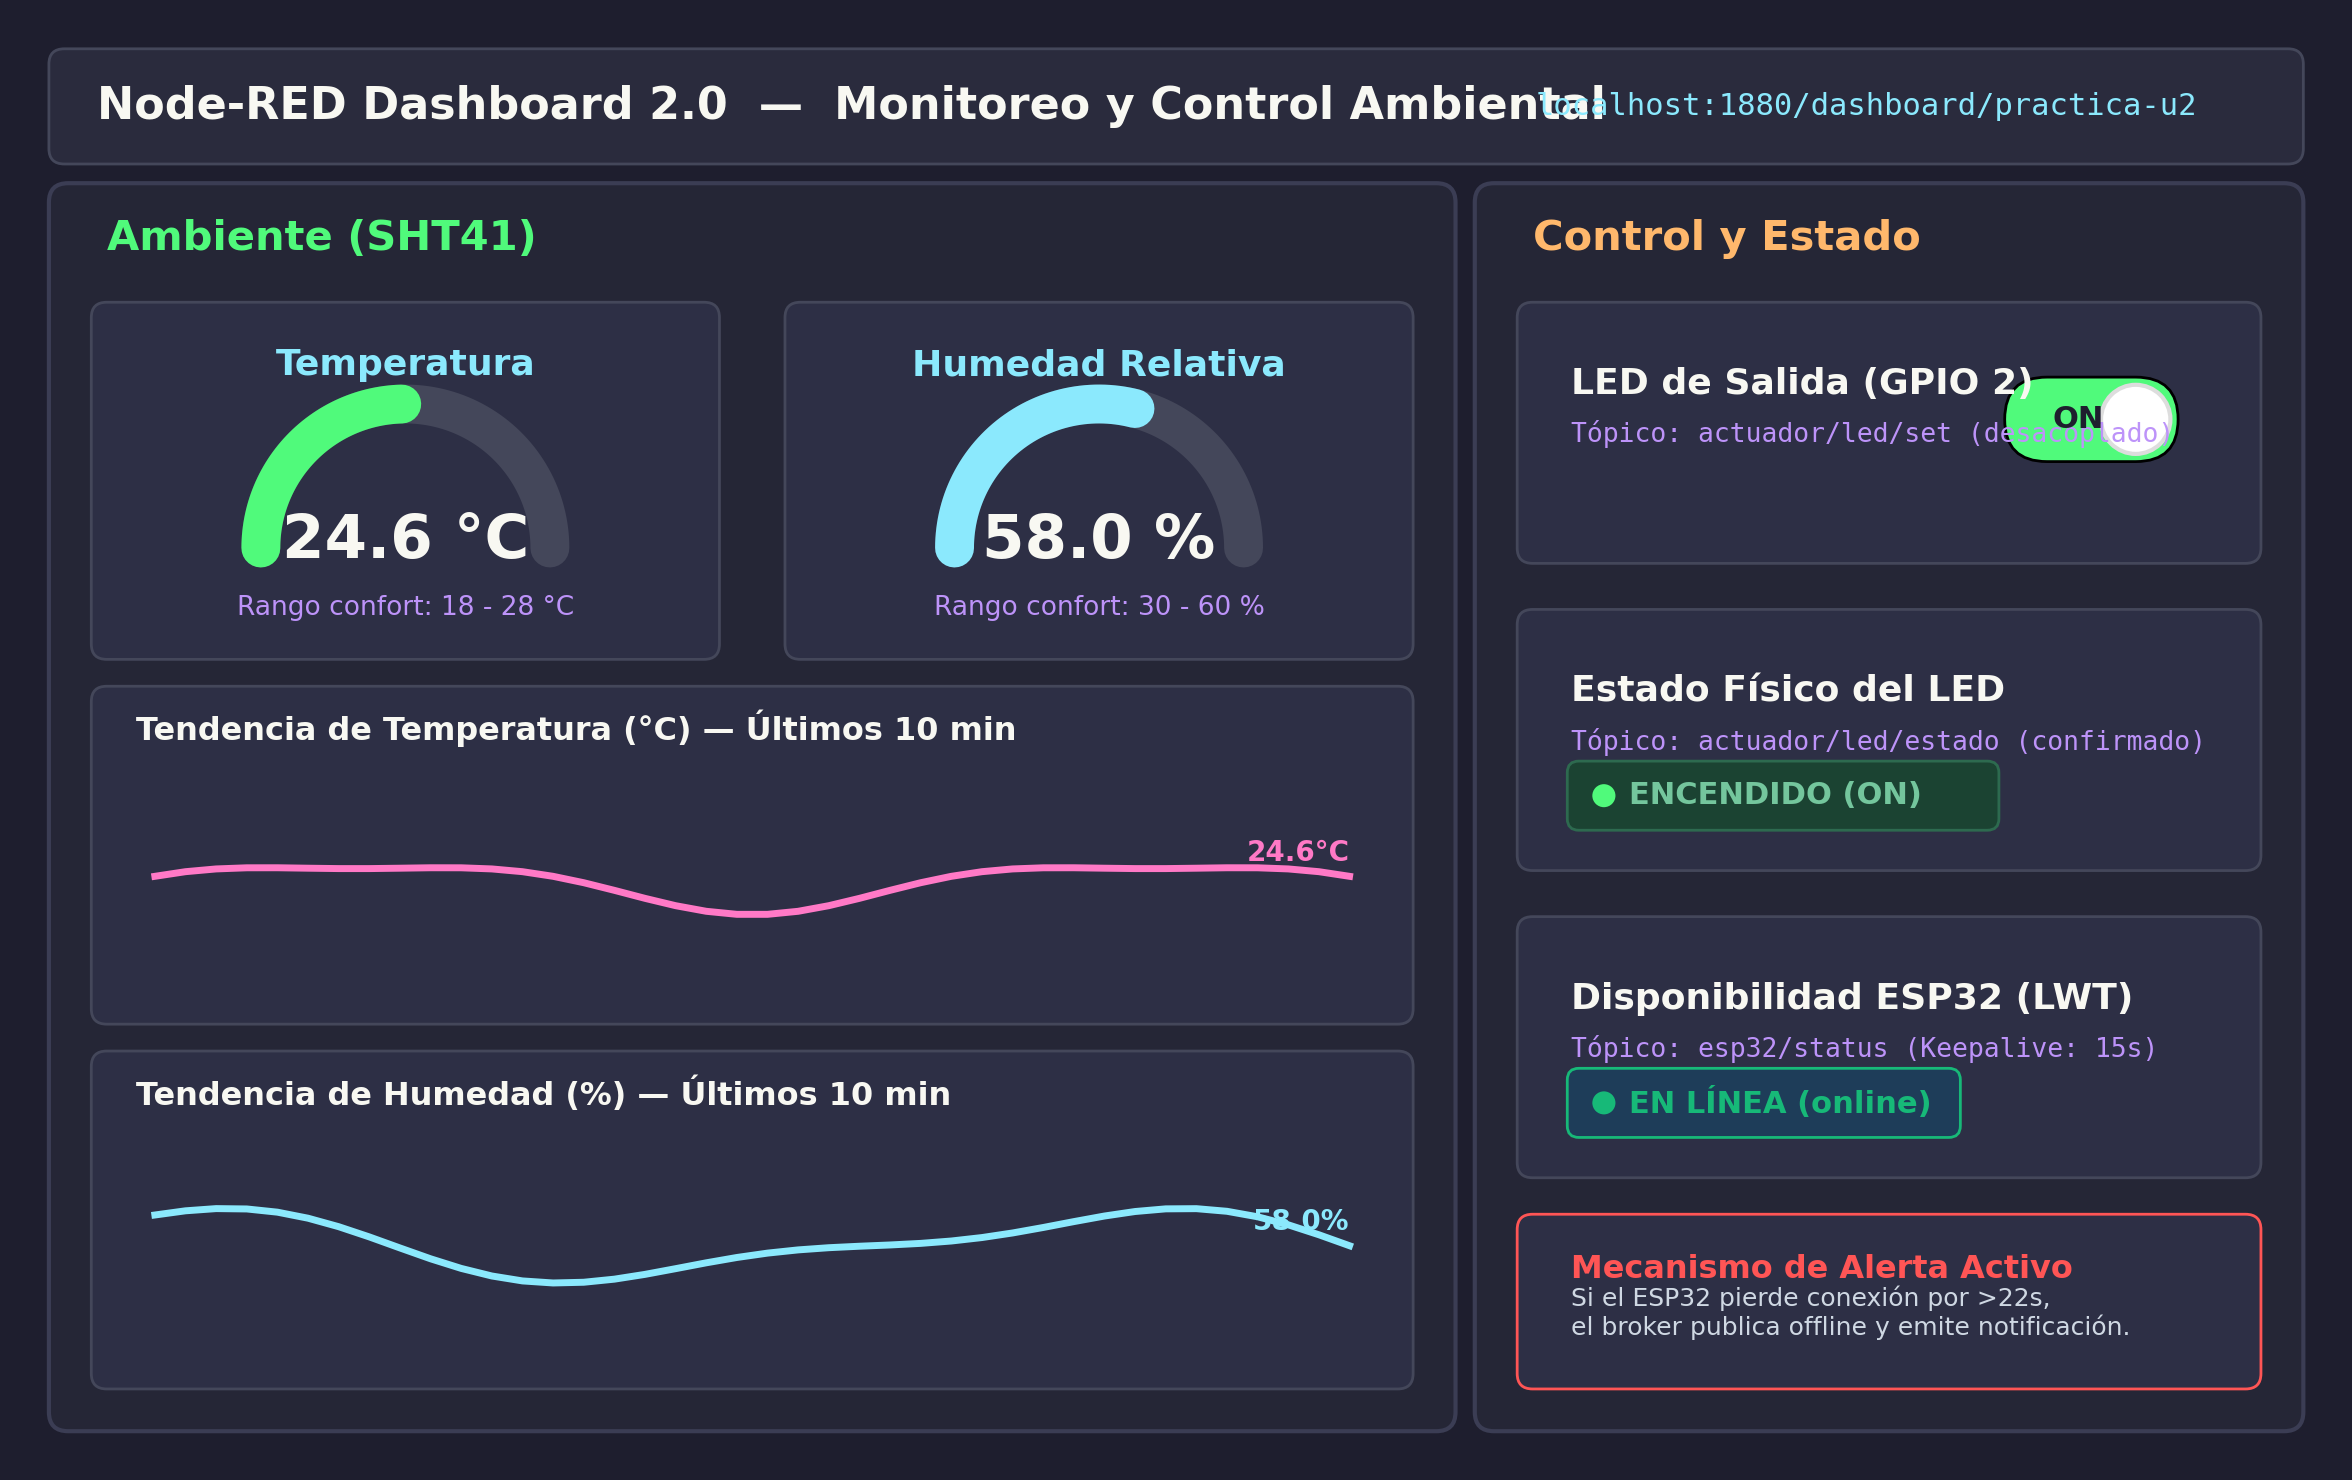
\includegraphics[width=\textwidth]{imagenes/dashboard_nodered.png}
        \caption{Dashboard 2.0 de Node-RED.}
        \label{fig:sub_dashboard}
    \end{subfigure}
    \caption{Evidencias de montaje físico y panel de supervisión web.}
    \label{fig:evidencias_visuales}
\end{figure}

\subsection{Demostración en Video}
\begin{infobox}[Video Demostrativo de Comunicación Bidireccional]
    \centering
    \textbf{Acceso al video demostrativo de pruebas experimentales:}\\
    \vspace{0.15cm}
    \url{https://drive.google.com/drive/folders/ejemplo-enlace-video-practica-u2}\\
    \vspace{0.15cm}
    \textit{\small(Demuestra la conmutación remota del LED, la actualización de la OLED y el reporte de LWT ante desconexiones).}
\end{infobox}

\subsection{Pruebas de Validación Experimental}
\begin{enumerate}
    \item \textbf{Secuencia de arranque en monitor serie (115200 bps):}
\begin{lstlisting}[style=custombash]
Conectando a WiFi: ESP32-Proyecto
WiFi conectado. IP del ESP32: 10.42.0.84
Conectando a broker MQTT... conectado.
Publicado en MQTT: {"temp":24.6,"hum":58.0}
Mensaje recibido [actuador/led/set]: ON
LED -> ON
\end{lstlisting}
    \item \textbf{Suscripción a telemetría desde terminal (CLI):}
\begin{lstlisting}[style=custombash]
$ mosquitto_sub -h 10.42.0.1 -u dashboard -P '<pass>' -v -t 'sensor/sht41/#' -t 'actuador/led/estado'
esp32/status online
actuador/led/estado OFF
sensor/sht41/temperatura 24.6
sensor/sht41/humedad 58.0
\end{lstlisting}
    \item \textbf{Control de actuador y confirmación de estado:} Al publicar \texttt{mosquitto\_pub -t actuador/led/set -m ON -q 1 -r}, el LED físico se enciende, la pantalla OLED muestra \texttt{LED:ON} y el ESP32 publica \texttt{actuador/led/estado ON}.
    \item \textbf{Verificación de LWT:} Al retirar la alimentación del ESP32, transcurridos 22 segundos el broker emite automáticamente \texttt{esp32/status offline}, actualizando el dashboard a \textbf{🔴 Desconectado}.
\end{enumerate}
